%
% Repeater Synchronisation
%

\section{Repeater synchronisation}\index{Repeater synchronisation}\index{Race-time condition}

When employing non-deterministic entanglement sources in a quantum repeater network\index{Quantum repeater network} there is no guarantee that pumping the source will actually yield an output entangled pair. Indeed this is extremely unlikely for sources such as SPDC. For this reason quantum memories will be required when performing entanglement swapping, so as to temporally synchronise the unpredictable arrival times of qubits.

However, future technologies may enable push-button entanglement sources\index{Push-button source}, in which case there is no ambiguity in the preparation times of pairs. In this instance quantum memories may be avoided entirely. Instead we can trigger all the sources at exactly the right times so as to ensure that at every joint measurement device in the repeater network the photons arrive simultaneously.

Consider a simple quantum repeater network, comprising a linear chain of alternating Bell-pair sources and entanglement swappers, as shown in Fig.~\ref{fig:racetime}.

\begin{figure*}[!htb]
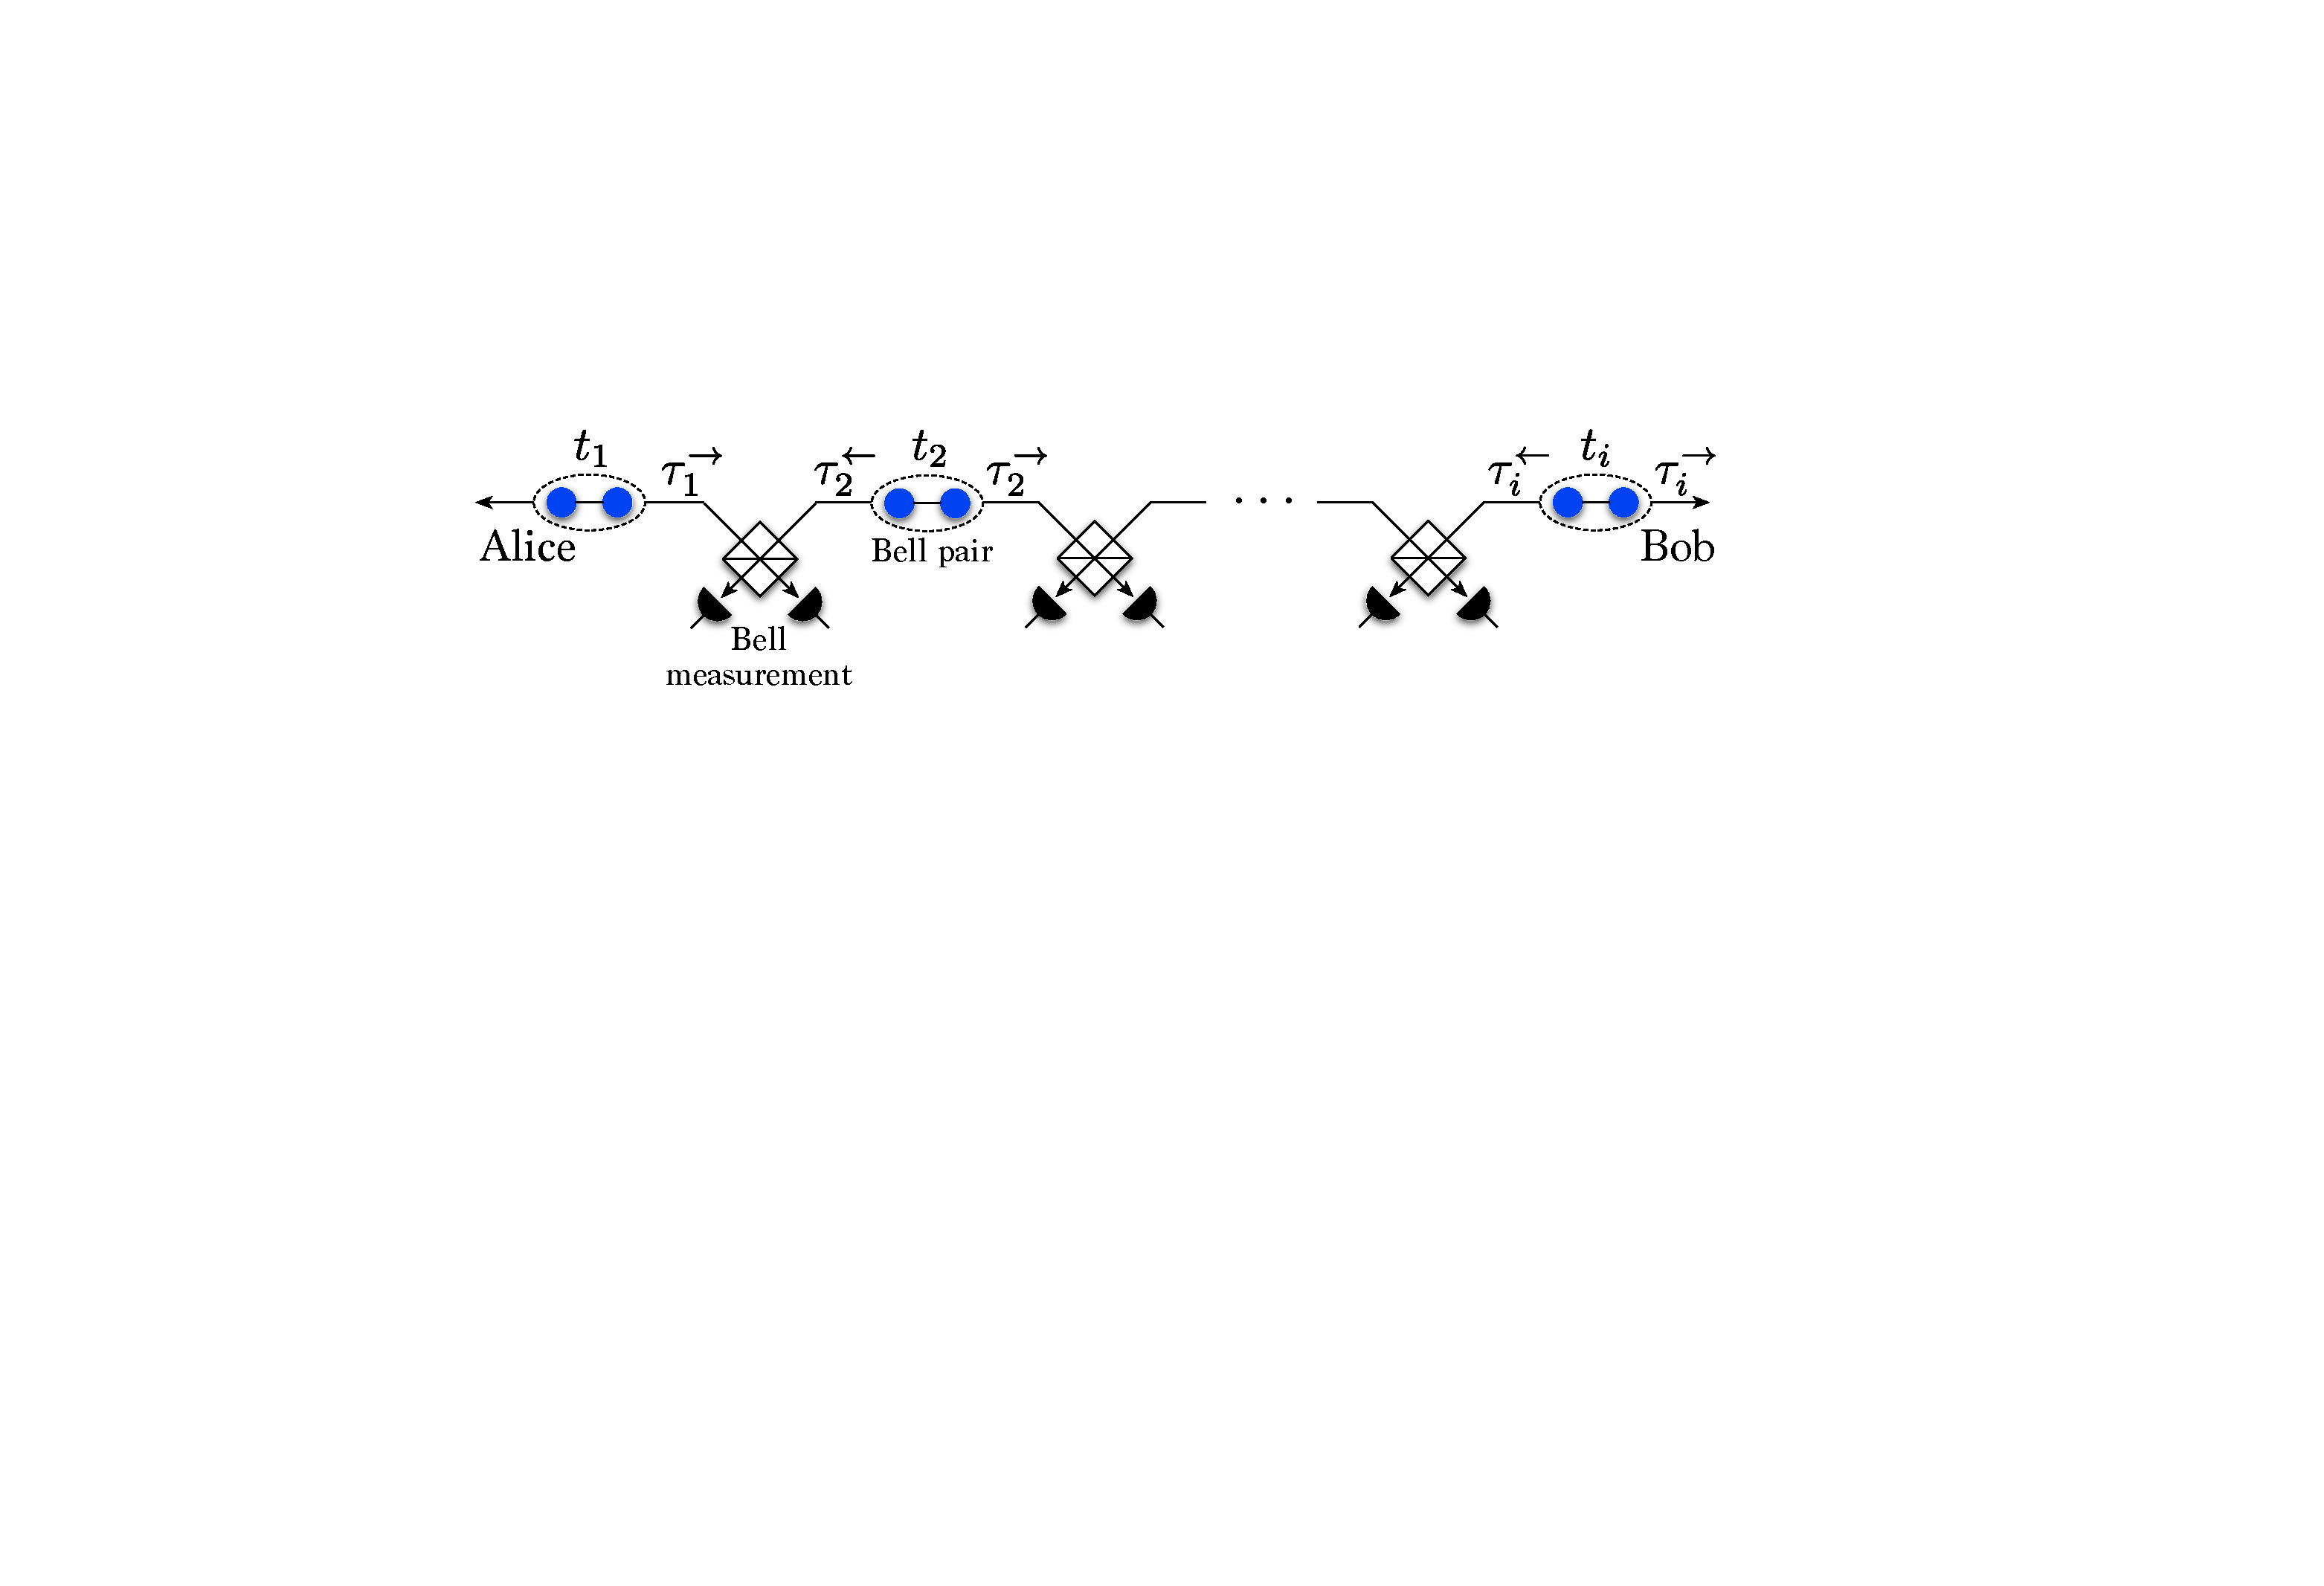
\includegraphics[width=\textwidth]{racetime}
\caption{A linear quantum repeater network comprising Bell-pair sources and Bell measurements. Upon success this yields a single Bell-pair between the leftmost and rightmost photonic qubits. $t_i$ is the triggering time of the $i$th source, and $\tau_i^\leftarrow$ ($\tau_i^\rightarrow$) are the channel propagation times between the $i$th source and the entanglement swapper to its immediate left (right). With push-button sources\index{Push-button source}, if the $t_i$ are chosen appropriately, as per Eq.~(\ref{eq:repeater_trig_time_sol}), we can satisfy the race-time condition\index{Race-time condition} of simultaneous arrival times of photons at Bell measurements, mitigating the need for quantum memories to synchronise them.}\label{fig:racetime}	
\end{figure*}

Let $t_i$ be the triggering time of the $i$th source, and $\tau_i^\leftarrow$ ($\tau_i^\rightarrow$) be the channel propagation times from the $i$th source to the entanglement swapper immediately to its left (right) in the chain. Imposing the race-time condition\index{Race-time condition} that two photons arriving at a measurement device are simultaneous,
\begin{align}\label{eq:ent_sync_cond}
t_i + \tau_i^\rightarrow &= t_{i+1} + \tau_{i+1}^\leftarrow,	
\end{align}
where we set \mbox{$t_1=0$} as a reference. This yields the linear system of equations,
\begin{align}
\hat{T}\cdot\vec{t} = \vec{\delta},
\end{align}
where,
\begin{align}
\hat{T} = \left[\begin{matrix}{}
 -1 & 0 & 0 & 0 &\dots \\
 1 & -1 & 0 & 0 & \\
 0 & 1 & -1 & 0 & \\
 0 & 0 & 1 & -1 & \\
 \vdots & & & & \ddots
\end{matrix}\right],
\end{align}
\begin{align}
\vec{t} = \left[\begin{matrix}{}
t_2\\
t_3\\
t_4\\
t_5\\
\vdots	
\end{matrix}\right],
\end{align}
\begin{align}
\vec\delta &= \left[\begin{matrix}{}
\tau_{2}^\leftarrow - \tau_1^\rightarrow	 \\
\tau_{3}^\leftarrow - \tau_2^\rightarrow	 \\
\tau_{4}^\leftarrow - \tau_3^\rightarrow	 \\
\tau_{5}^\leftarrow - \tau_4^\rightarrow	 \\
\vdots
\end{matrix}\right].
\end{align}
Solving,
\begin{align}\label{eq:repeater_trig_time_sol}
	\vec{t} = \hat{T}^{-1}\cdot\vec\delta,
\end{align}
where,
\begin{align}
	\hat{T}^{-1} & = \left[\begin{matrix}{}
 -1 & 0 & 0 & 0 &\dots \\
 -1 & -1 & 0 & 0 & \\
 -1 & -1 & -1 & 0 & \\
 -1 & -1 & -1 & -1 & \\
 \vdots & & & & \ddots
\end{matrix}\right],
\end{align}
yields the required triggering times for all sources (relative to \mbox{$t_1=0$}) to ensure synchronisation of photon arrival times at all entanglement swappers.